\documentclass[12pt]{article}
\usepackage{Style-Thesis-Report}

% You can define your own commands like this
\newcommand{\um}{$\upmu$m} % easily creates the label for ``micrometers''




\begin{document}
	
\begin{titlepage}
	\begin{center}
		
		\vspace*{1cm}
		
		\Huge
		\textbf{Compton Scattering - Report 1}
		\large
		\vspace{1.5cm}
		
		Yacine Benkirane\\
		Eloise Chakour\\
		Yukuan Zhao\\
		
		McGill University Department of Physics
		
		Supervisor: Prof. Thomas Brunner and Prof. Dominic Ryan
		
		\today
		
	\end{center}
	
\end{titlepage}

\begin{abstract}

Abstract This file is already set up with the correct margins, font, and line spacing. It is designed to show examples of how to create and organize a LaTeX document. Simply make a copy of this tex file and then overwrite all of the nonsense with your own content. If this gives you trouble, or you're just annoyed with LaTeX, I highly recommend using LyX instead. LyX is based on latex, but you don't have to look at the underlying code (though you can if you want!). This means everything you learn and do in LyX (especially equations!) will be easier, and can be directly applied / copied / pasted to a latex document, should you go this route in the future. If you stick with LaTeX, I can say from experience that TeXstudio is the best editor I've seen.

\end{abstract}
\tableofcontents{}

\thispagestyle{empty}
\pagebreak
\setcounter{page}{1}


\section{Test Section}\label{sec:test}

You can write a section intro here. Section \ref{sec:sub} below shows a demo of a subsection.

This is a new paragraph, with some $M_\textrm{ath}=I_n lin_e$, and a larger equation can be made as follows:
%
\begin{equation}\label{eq:pants}
ax^2 + bx + c = 0
\end{equation}
%
Sadly, Eq.~\ref{eq:pants} is super boring. Note the little \% symbols in the latex code. They prevent a new paragraph from forming.



\subsection{Test Subsection}\label{sec:sub}

You can also do subsubsections if you really want. 

\begin{figure}
	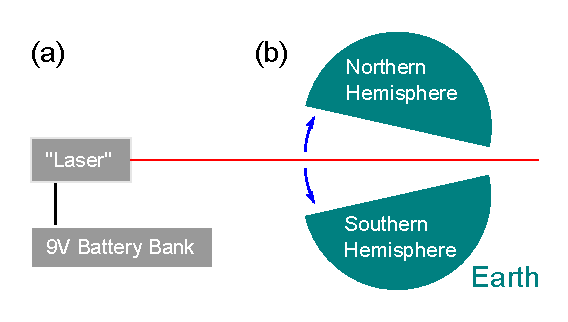
\includegraphics[width=12cm]{Figures/Figure1.pdf}
	\caption{Space Laser Facility and action upon earth. (a) Space laser facility: A bank of $10^{18}$ 9V batteries powers the primary laser. (b) The laser output is swept along the equator from east to west at a rate of 5 radians / hour, producing a clean split between the northern and southern hemispheres. }
	\label{fig:laser}
\end{figure}

Figure \ref{fig:laser}(a) shows a simplified drawing of the Space Laser Facility (SPL). A bank of $10^{18}$ 9-volt batteries (Eveready \textregistered X-treme bulkbox) supplies power to a sophisticated heat beam known as a ``Laser''. In Fig.~\ref{fig:laser}(b), we show the estimated response of earth for a laser swept along the equator at a rate of 5 radians / hour from east to west. Blue arrows indicate the approximate direction of motion. Due to the rotation of the earth, a similar sweep from west to east will not produce a clean cut \cite{Sankey2010Strong}. The wavelength of this laser, $\lambda=1.55$ \um, is chosen primarily because the telecom industry has produced a multitude of low-cost components at this wavelength.



We definitely recommend using Mendeley to organize your citations and generate a bibliography file. You can set this up so that from the abstract page online, you can click a button that adds it to your library. Then it's just a matter of exporting to ``bibtex'' format.




% Bibliography:
\bibliographystyle{IEEEtran}
\bibliography{MyBibliography}

\end{document}